%File: anonymous-submission-latex-2024.tex
\documentclass[letterpaper]{article} % DO NOT CHANGE THIS
\usepackage[submission]{aaai24}  % DO NOT CHANGE THIS
\usepackage{times}  % DO NOT CHANGE THIS
\usepackage{helvet}  % DO NOT CHANGE THIS
\usepackage{courier}  % DO NOT CHANGE THIS
\usepackage[hyphens]{url}  % DO NOT CHANGE THIS
\usepackage{graphicx} % DO NOT CHANGE THIS
\urlstyle{rm} % DO NOT CHANGE THIS
\def\UrlFont{\rm}  % DO NOT CHANGE THIS
\usepackage{natbib}  % DO NOT CHANGE THIS AND DO NOT ADD ANY OPTIONS TO IT
\usepackage{caption} % DO NOT CHANGE THIS AND DO NOT ADD ANY OPTIONS TO IT
\frenchspacing  % DO NOT CHANGE THIS
\setlength{\pdfpagewidth}{8.5in} % DO NOT CHANGE THIS
\setlength{\pdfpageheight}{11in} % DO NOT CHANGE THIS
%
% These are recommended to typeset algorithms but not required. See the subsubsection on algorithms. Remove them if you don't have algorithms in your paper.
\usepackage{algorithm}
\usepackage{algorithmic}
\usepackage{amsmath}
\usepackage{mathtools}
\usepackage[usestackEOL]{stackengine}
\stackMath
%
% These are are recommended to typeset listings but not required. See the subsubsection on listing. Remove this block if you don't have listings in your paper.
\usepackage{newfloat}
\usepackage{listings}
\DeclareCaptionStyle{ruled}{labelfont=normalfont,labelsep=colon,strut=off} % DO NOT CHANGE THIS
\lstset{%
	basicstyle={\footnotesize\ttfamily},% footnotesize acceptable for monospace
	numbers=left,numberstyle=\footnotesize,xleftmargin=2em,% show line numbers, remove this entire line if you don't want the numbers.
	aboveskip=0pt,belowskip=0pt,%
	showstringspaces=false,tabsize=2,breaklines=true}
\floatstyle{ruled}
\newfloat{listing}{tb}{lst}{}
\floatname{listing}{Listing}
%
% Keep the \pdfinfo as shown here. There's no need
% for you to add the /Title and /Author tags.
\pdfinfo{
/TemplateVersion (2024.1)
}

\setcounter{secnumdepth}{2} %May be changed to 1 or 2 if section numbers are desired.

% The file aaai24.sty is the style file for AAAI Press
% proceedings, working notes, and technical reports.
%

% Sarus defined packages and commands
% A command for the project name
\usepackage{amsfonts}
\usepackage{xcolor}
\newcommand{\qrlew}{\emph{Qrlew}}
\newcommand{\commentNG}[1]{{\color{red}[NG: {#1}]}}
\newcommand{\commentPR}[1]{{\color{green}[PR: {#1}]}}
\newcommand{\commentVdSA}[1]{{\color{blue}[VdSA: {#1}]}}


\newcommand\coolover[2]{\mathrlap{\smash{\overbrace{\phantom{%
    \begin{matrix} #2 \end{matrix}}}^{\mbox{$#1$}}}}#2}

\newcommand\coolrightbrace[2]{%
\left.\vphantom{\begin{matrix} #1 \end{matrix}}\right\}#2}

% Title

% Your title must be in mixed case, not sentence case.
% That means all verbs (including short verbs like be, is, using,and go),
% nouns, adverbs, adjectives should be capitalized, including both words in hyphenated terms, while
% articles, conjunctions, and prepositions are lower case unless they
% directly follow a colon or long dash
\title{\qrlew: Query Rewriting for Differential Privacy}
\author{
    %Authors
    % Authors
    Nicolas Grislain\textsuperscript{\rm 1}
    Paul Roussel\textsuperscript{\rm 1}
    Victoria de Sainte Agathe\textsuperscript{\rm 1}
}
\affiliations{
    %Afiliations
    \textsuperscript{\rm 1}Sarus Technologies\\
    % If you have multiple authors and multiple affiliations
    % use superscripts in text and roman font to identify them.
    % For example,

    % Sunil Issar\textsuperscript{\rm 2},
    % J. Scott Penberthy\textsuperscript{\rm 3},
    % George Ferguson\textsuperscript{\rm 4},
    % Hans Guesgen\textsuperscript{\rm 5}
    % Note that the comma should be placed after the superscript

    1900 Embarcadero Road, Suite 101\\
    Palo Alto, California 94303-3310 USA\\
    % email address must be in roman text type, not monospace or sans serif
    proceedings-questions@aaai.org
%
% See more examples next
}

\iffalse
%Example, Multiple Authors, ->> remove \iffalse,\fi and place them surrounding AAAI title to use it
\title{\qrlew: automatic differential privacy for SQL queries}
\author {
    % Authors
    Nicolas Grislain,
    Paul Roussel,
    Victoria de Sainte Agathe,
}
\affiliations {
    % Affiliations
    ng@sarus.tech, pr@sarus.tech, vdsa@sarus.tech
}
\fi

\begin{document}

\maketitle

\begin{abstract}
This paper introduces \qrlew{}, an \emph{open source} library that can parse SQL queries into \emph{Relations} --- an intermediate representation --- that keeps track of rich data types, value ranges, and row ownershi; so that they can easily be rewritten into \emph{differentially-private} equivalent and turned back into SQL queries for execution in a variety of standard data stores.

With \qrlew{}, a \emph{data practitionner} can express their data queries in standard SQL; the \emph{data owner} can run the rewritten query without any technical integration and with strong privacy garantees on the output; and the query rewriting can be operated by a privacy-expert who must be trusted by the owner, but may belong to a separate organizations.
\end{abstract}

\section{Introduction}

In recent years, the importance of safeguarding privacy when dealing with personal data has continuously increased.
Traditional anonymization techniques have proven vulnerable to re-identification, as demonstrated by numerous works \cite{archie2018s, dwork2017exposed, narayanan2008robust, sweeney2013identifying}.
The total cost of data breaches has also significantly increased \cite{ibm2023cost} and governments have introduced stricter data protection laws.
Yet, the collection, sharing, and utilization of data hold the potential to generate significant value across various industries, including healthcare, finance, transportation, and energy distribution.

To realize these benefits while managing privacy risks, researchers have turned to \emph{differential privacy (DP)} \cite{wood2018differential, dwork2014algorithmic}, which has become the \emph{gold standard} for privacy protection since its introduction by Dwork et al. in 2006 \cite{dwork2006calibrating} due to its provable and automatic privacy guarantees.

Despite the availability of powerful open-source tools \cite{kotsogiannis2019privatesql, diffprivlib, OpenDP, PipelineDP, ZetaSQL, PrivacyOnBeam, johnson2020chorus, berghel2022tumult, yousefpour2021opacus}, DP adoption remained limited and many organizations sticked to more manual and \emph{ad-hoc} approaches.
Reasons for this lack of adoption are probably complex and multiple but one could name: the lack of awareness on privacy risks; the loss of utility in the results; and the perceived complexity of the existing solutions considering they all require, either some expertise in differential privacy, or the use of new interfaces to express data processing tasks, or even to integrate new execution engines in their data stack.
\qrlew{} \cite{Grislain_Qrlew_2023} has been designed to relieve these problems by providing the following features:
\begin{description}
    \item[\qrlew{} provides automatic output privacy guarantees]
    With \qrlew{} a \emph{data owner} can let an analyst (\emph{data practitionner}) with no expertise in privacy protection run arbitrary SQL queries with strong privacy garantees on the output.
    \item[\qrlew{} leverages existing infrastructures]
    \qrlew{} rewrites a SQL query into a \emph{differentially private} SQL query that can be run on any data-store with a SQL interface: from lightweight DB to big-data stores.
This removes the need for a custom execution engine and enables \emph{differentially private analytics with virtually no technical integration}.
    \item[\qrlew{} leverages synthetic data]
    Synthetic data are an increasingly popular way of \emph{privatizing} a dataset. Using jointly: \emph{differentially private} mechanisms and \emph{differentially private} synthetic data can be a simple, yet powerful, way of managing a privacy budget and reaching better utility-privacy tradeoffs.
\end{description}

% Motivation DP
% Solutions existantes
% Problème non résolu et nécessité de \qrlew

% à développer plus:
% - adaptativité -> utiliser output DP pour tuner DP aval
% - More mechanisms
% - Interconnectivité
\section{Definitions}

\subsection*{Datasets and Protected Entities (PE)}

In this paper, \emph{datasets} refers to a collection of elements in some domain $\mathcal{X}$, labelled by an identifier $i\in \mathcal{I}$ identifying the entity whose privacy we want to protect. This entity will be called \emph{Protected Entity} (PE) and the identifier will be referd to as \emph{Protected Entity ID} (PEID). Let $\mathcal{D}$ be the set of datasets of arbitrary sizes with a protected entity.

\subsection*{Differential Privacy (DP)}

Let $\mathcal{M}$ be an algorithm that takes a dataset as input and produces a randomized output. The algorithm $\mathcal{M}$ is said to satisfy $\varepsilon,\delta$-differential privacy if, for all pairs of adjacent datasets $D, D' \in \mathcal{D}$, and for all measurable sets $S$ in the range of $\mathcal{M}$:
$$\Pr[\mathcal{M}(D) \in S] \leq e^{\varepsilon} \cdot \Pr[\mathcal{M}(D') \in S] + \delta$$

\subsection*{Adjacent datasets}

Datasets $D, D' \in \mathcal{D}$ are adjacent if they are equal up to the addition or removal of all entries sharing the same PEID. Note that this is a slightly unusual and restricted definition of adjacency, suited to our practical needs. It is close to that used in the \emph{user-level differential privacy} literature \cite{liu2020learning, wilson2019differentially} where one user can have many samples.

\section{Assumptions and Design Goals}

In this work, we assume the \emph{central model of differential privacy} \cite{near2020threat}, where a trusted central organization: hospital, insurance company, utility provider, called the \emph{data owner}, collects and stores personal data in a secure database and whishes to let untrusted \emph{data practitionners} run SQL queries on its data.

At a high level we pursued the following requirements:
\begin{itemize}
    \item Ease of use for the \emph{data practitionners}. The \emph{data practitionners} are assumed to be a data experts but no privacy experts. They should be able to express their queries in a standard way. We chose SQL as the query language as it is very commonly used for analytics tasks.
    \item Ease of integration for the \emph{data owner}. As SQL is a common language to express data analysis tasks, many data-stores support it from small embedded databases to big data stores.
    \item Simplicity for the \emph{data owner} to setup privacy protection. Differential privacy is about capping the sensitivity of a result to the addition or removal of an individual that we call \emph{protected entity}. \qrlew{} assumes that the \emph{data owner} can tell if a table is public and, if it is not, that it can assign exactly one \emph{protected entity} to each row of data. In the case there are multiple related tables, \qrlew{} enables to define easily the \emph{protected entities} for each tables transitively.
    \item Simple integration with other privacy enhancing technologies such as \emph{synthetic data}. To avoid repeated privacy losses or give result when a DP rewriting is not easily available (e.g. when the query is: \texttt{SELECT * FROM table}) \qrlew{} can use \emph{synthetic data} to blend in the computation.
\end{itemize}

These requirements dictated the overall \emph{query rewriting} architecture and many features, the most important of which, are detailed bellow.

\section{Architecture and main features of \qrlew}

The \qrlew{} library, solves the problem of running a SQL query with DP guarantees in three steps. First the SQL query submitted by the \emph{data practitionner} is parsed and converted into a \emph{Relation}, this \emph{Relation} is an intermediate representation that is designed to ease the tracking of data types ranges or possible values, to ease the tracking of the \emph{protected entity} and to ease the rewriting into a DP \emph{Relation}. Then, the rewritting into DP happens. Once the relation is rewriten into a DP one, it can be rendered as an SQL query string and submited to the data store of the \emph{data owner}. The output can then safely be shared with the \emph{data practitionner}. This process is illustrated in Figure~\ref{fig:process}.

\begin{figure*}[t]
    \centering
    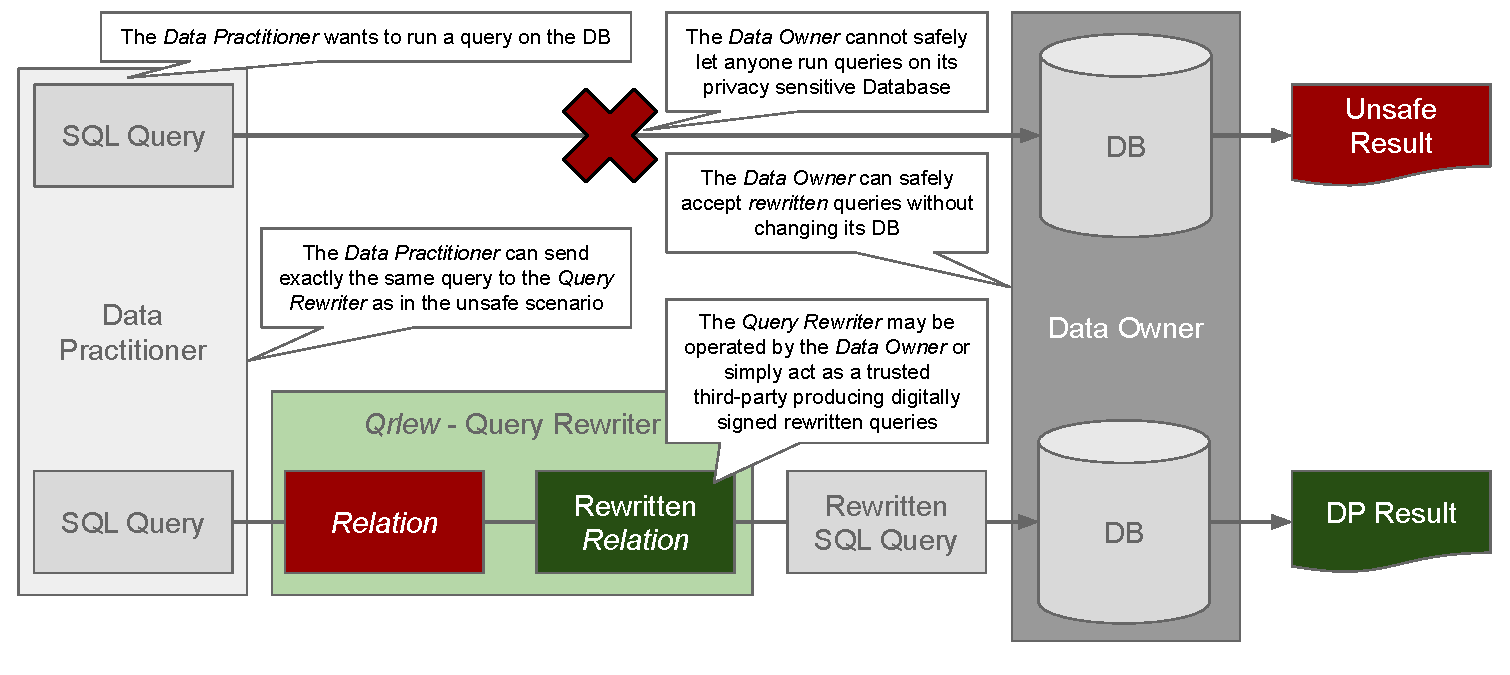
\includegraphics[width=0.9\textwidth]{figures/qrlew_process} % Reduce the figure size so that it is slightly narrower than the column.
    \caption{The rewritting process occurs in three stages: The \emph{data practitionner}'s query is parsed into a \emph{Relation}, which is rewritten into a DP equivalent and finally executed by the the \emph{data owner} which returns the privacy-safe result.}
    \label{fig:process}
\end{figure*}

\subsection{Qrlew Intermediate Representation}

As the SQL language is very rich and complex, simply parsing a query into an abstract syntaxic tree does not produce a convenient representation for our needs. Therefore, it is converted into a simpler normalized representation with properties well aligned with the requirements of Differential Privacy: the \emph{Relation}. A \emph{Relation} is a collection of rows adhering to a given \emph{schema}. It is a recursively defined structure composed of:
\begin{description}
    \item[\emph{Tables}] This is simply a data source from a database.
    \item[\emph{Maps}] A \emph{Map} takes an input \emph{Relation}, filters the rows and transform them one by one. The filtering conditions and row transforms are expressed with expressions similar to those of SQL. It acts as a \texttt{SELECT exprs FROM input WHERE expr LIMIT value} and therefore preserve the \emph{protected entity} ownership structure.
    \item[\emph{Reduces}] A \emph{Reduce} takes an input \emph{Relation} and aggregates some columns, possibly group by group. It acts as a \texttt{SELECT aggregates FROM input GROUP BY expr}. This is where the rewriting into DP will happen as described in section~\ref{sec:rewritting}.
    \item[\emph{Joins}] This \emph{Relation} combines two input \emph{Relations} as a \texttt{SELECT * FROM left JOIN right ON expr} would do it. The privacy properties are more complex to propagate in this case.
\end{description}
It may also be a static list of values or a set operation between two \emph{Relations}, but those are less important for our uses.

\begin{figure}[t]
    \centering
    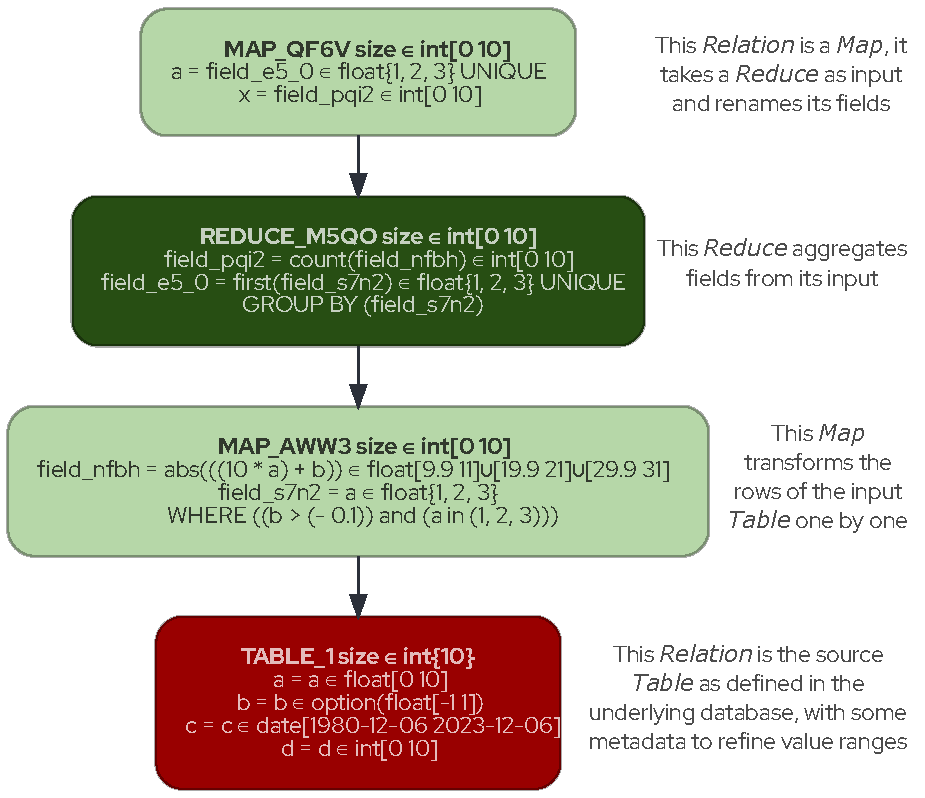
\includegraphics[width=0.4\textwidth]{figures/relation}
    \caption{\emph{Relation} (\emph{Map}) associeted to the query: \texttt{SELECT a, count(abs(10*a+b)) AS x FROM table\_1 WHERE b>-0.1 AND a IN (1,2,3) GROUP BY a}. The arrows point to the inputs of each \emph{Relation}. Note the propagation of the data type ranges.}
    \label{process}
\end{figure}

This representation is central to \qrlew{}; all the features described below are built upon it. A \emph{Relation} along with all the  sub-\emph{Relations} it is depending on, will be called the \emph{computation graph} or the \emph{graph} of a \emph{Relation}.

\subsection{Range Propagation}

Most DP mechanisms aggregating numbers require the knowledge of some bounds on the values (see \cite{dwork2014algorithmic}).
Even if some bounds are known for some \emph{Relations} like source \emph{Tables}, it is not trivial to propagate these bounds through the steps of the computation.

To help with range propagation, \qrlew{} introduces two useful concepts:
\begin{itemize}
    \item The concept of \emph{$k$-Interval}, which are finite union of at most $k$ closed intervals. A \emph{$k$-Interval} can be noted:
    $$I = \bigcup_{i=1}^{j\leq k}\left[a_i, b_i\right]$$
    Note that the union of \emph{$k$-Interval}s may not be a \emph{$k$-Interval} as it may be the union of more than $k$ intervals.
    Unions of many intervals can be simplified into their convex enveloppe interval, which are often sufficient bounds approximations for our use cases:
    $$J = \bigcup_{i=1}^{j> k}\left[a_i, b_i\right] \subseteq \left[\min_i a_i, \max_i b_i\right]$$
    \item The concept of \emph{piecewise-monotonic-functions}\footnote{Which is a shorthand name for what would be better called: \emph{piecewise-coordinatewise-monotonic-functions}}, which are functions $f: \mathbb{R}^n \rightarrow \mathbb{R}$ whose domain can be partitioned in cartesian products of intervals $P_j$ on which they are \emph{coordinatewise-monotonic}.
    The image of a cartesian product of $n$ \emph{$k$-Interval}s by a \emph{piecewise-monotonic-function} can be easily computed as a \emph{$k$-Interval}.
    Indeed, let $I$ be:
    $$I = I_1\times I_2\times \ldots \times I_n = \bigcup_{\substack{1\leq i_1\leq k\\\ldots\\1\leq i_n\leq k}}\left[a_{i_1}, b_{i_1}\right]\times \ldots \times \left[a_{i_n}, b_{i_n}\right]$$
    If $f$ is \emph{piecewise-monotonic}, then one can show that on each partition $P_j$ where it is \emph{coordinatewise-monotonic}, if we note:
    $$I_j = I \cap P_j = \bigcup_{\substack{1\leq j_1\leq k\\\ldots\\1\leq j_n\leq k}}\left[a_{j_1}, b_{j_1}\right]\times \ldots \times \left[a_{j_n}, b_{j_n}\right]$$
    $$f(I_j) = \bigcup_{\substack{1\leq i_1\leq k\\\ldots\\1\leq i_n\leq k}}\text{Conv}\left(f\left( \left\{a_{i_1}, b_{i_1}\right\}\times \ldots \times \left\{a_{i_n}, b_{i_n}\right\}\right)\right)$$
    where $\text{Conv}\left(f\left( \left\{a_{i_1}, b_{i_1}\right\}\times \ldots \times \left\{a_{i_n}, b_{i_n}\right\}\right)\right)$ can be efficiently computed in $n$ steps, without testing all the $2^n$ combinantions, thanks to the coordinatewise monotony of $f$ on $P_j$.
    Then $f(I) = \bigcup_j f(I_j)$, of which we can derive the bounding: $f(I) \subseteq \text{Conv}\left(\bigcup_j f(I_j)\right)$ when the number of terms in the union exceeds $k$.
\end{itemize}

The notion of \emph{$k$-Interval} is convenient for tracking value bounds as it can express natural patterns in SQL such as:
\begin{itemize}
    \item \texttt{WHERE x>0 AND x<=1}, which translates into the implied $x\in \left[0, 1\right]$ ;
    \item \texttt{WHERE x IN (1,2,3)}, which is also easily expressed as a \emph{k-Interval}: $x \in \left[1, 1\right] \cup \left[2, 2\right] \cup \left[3, 3\right]$
\end{itemize}

The idea of \emph{piecewise-monotonic-function} is also very useful as in SQL many standard arithmetic operators (\texttt{+}, \texttt{-}, \texttt{*}, \texttt{/}, \texttt{<}, \texttt{>}, \texttt{=}, \texttt{!=}, \ldots) and functions (\texttt{EXP}, \texttt{LOG}, \texttt{ABS}, \texttt{SIN}, \texttt{COS}, \texttt{LEAST}, \texttt{GREATEST}, \ldots) are trivially \emph{piecewise-monotonic-function} (in one, two or many variables).

Most of the range propagation in \qrlew{} is based on these concepts. It enables a rather simple and efficient range propagation mechanism, leading to better utility / privacy tradeoffs.

\subsection{Protected Entity Definition}

Tables in a database rarely come properly formated for privacy-preserving applications. Many rows in many tables may refer to the same individual, hence, \emph{adding or removing an individual} means \emph{adding or removing many rows}. To help the definition of the protected entity \qrlew{} introduces a small PE description language.
As examplified in listing~\ref{lst:pe}, PE definition associates to each private table in a database a path defining the PEID of each row. For a table containing the PE itself, like a \texttt{users} table for example, the PE definition will look like \texttt{("users",[],"id"),} where \texttt{id} is the name of a column identifying the user, like its name. If the database defines tables related to this tables, the way the tables are related should be specified following this scheme: $(\mathtt{tab}_1, path, \mathtt{peid})$ where $\mathtt{tab}_1$ is the name of the table for which the PEID is defined, $\mathtt{peid}$ is the name of the column defining the PEID in the table referred by $path$ and $path$ is a list of elements of the form $[(\mathtt{ref}_1, \mathtt{tab}_2, \mathtt{id}_2),\ldots, (\mathtt{ref}_{m-1}, \mathtt{tab}_m, \mathtt{id}_m)]$
where $\mathtt{ref}_{i-1}$ is a column in $\mathtt{tab}_{i-1}$ --- usually a foreign key --- referring to $\mathtt{tab}_i$ with a column of referred id $\mathtt{id}_i$ --- usually a primary key. Following the path of tables referring to one another, we end up with the table defining the PEID (e.g. \texttt{users}).

This small PE description language allows for a variety of usefull PEID scenarii, beyond the simple, but restrictive \emph{privacy per row}.

\begin{listing}[tb]
\caption{Example of \emph{protected entity} definition for a database with three tables holding users, orders and items records. Each user is protected individually by designating their \texttt{id}s as PEID. Orders are attached to a user through the foreigh key: \texttt{user\_id}. Items's ownership is defined the same way by specifying the lineage: \texttt{item -> order -> user}.}%
\label{lst:pe}
\begin{lstlisting}[language=Python]
protected_entity = [
  ("users",[],"id"),
  ("orders",[
    ("user_id","users","id")
  ],"id"),
  ("items",[
    ("order_id","orders","id"),
    ("user_id", "users", "id")
  ],"id")
]
\end{lstlisting}
\end{listing}

\subsection{Rewriting}
\label{sec:rewritting}

Rewriting in \qrlew{}, refers to the process of altering the \emph{computation graph} by substituting computation \emph{sub-graphs} to \emph{Relations} (see figure~\ref{fig:rewriting}) to alter the properties of the result. This substitution aims to achieve specific objectives, such as ensuring privacy through the incorporation of differentially private mechanisms. The rewriting process happens in two phases:
\begin{itemize}
    \item a \emph{rewriting rule allocation} phase, where each \emph{Relation} in the \emph{computation graph} gets allocated a \emph{rewriting rule} (RR) compatible with its input and with the desired output property
\end{itemize}
To facilitate this work, each \emph{Relation} is assigned a \emph{rewritting rule} that depends on the \emph{rewritting rules} (RR) of its input and then each \emph{Relation} is rewriten independently.

\begin{figure*}[t]
    \centering
    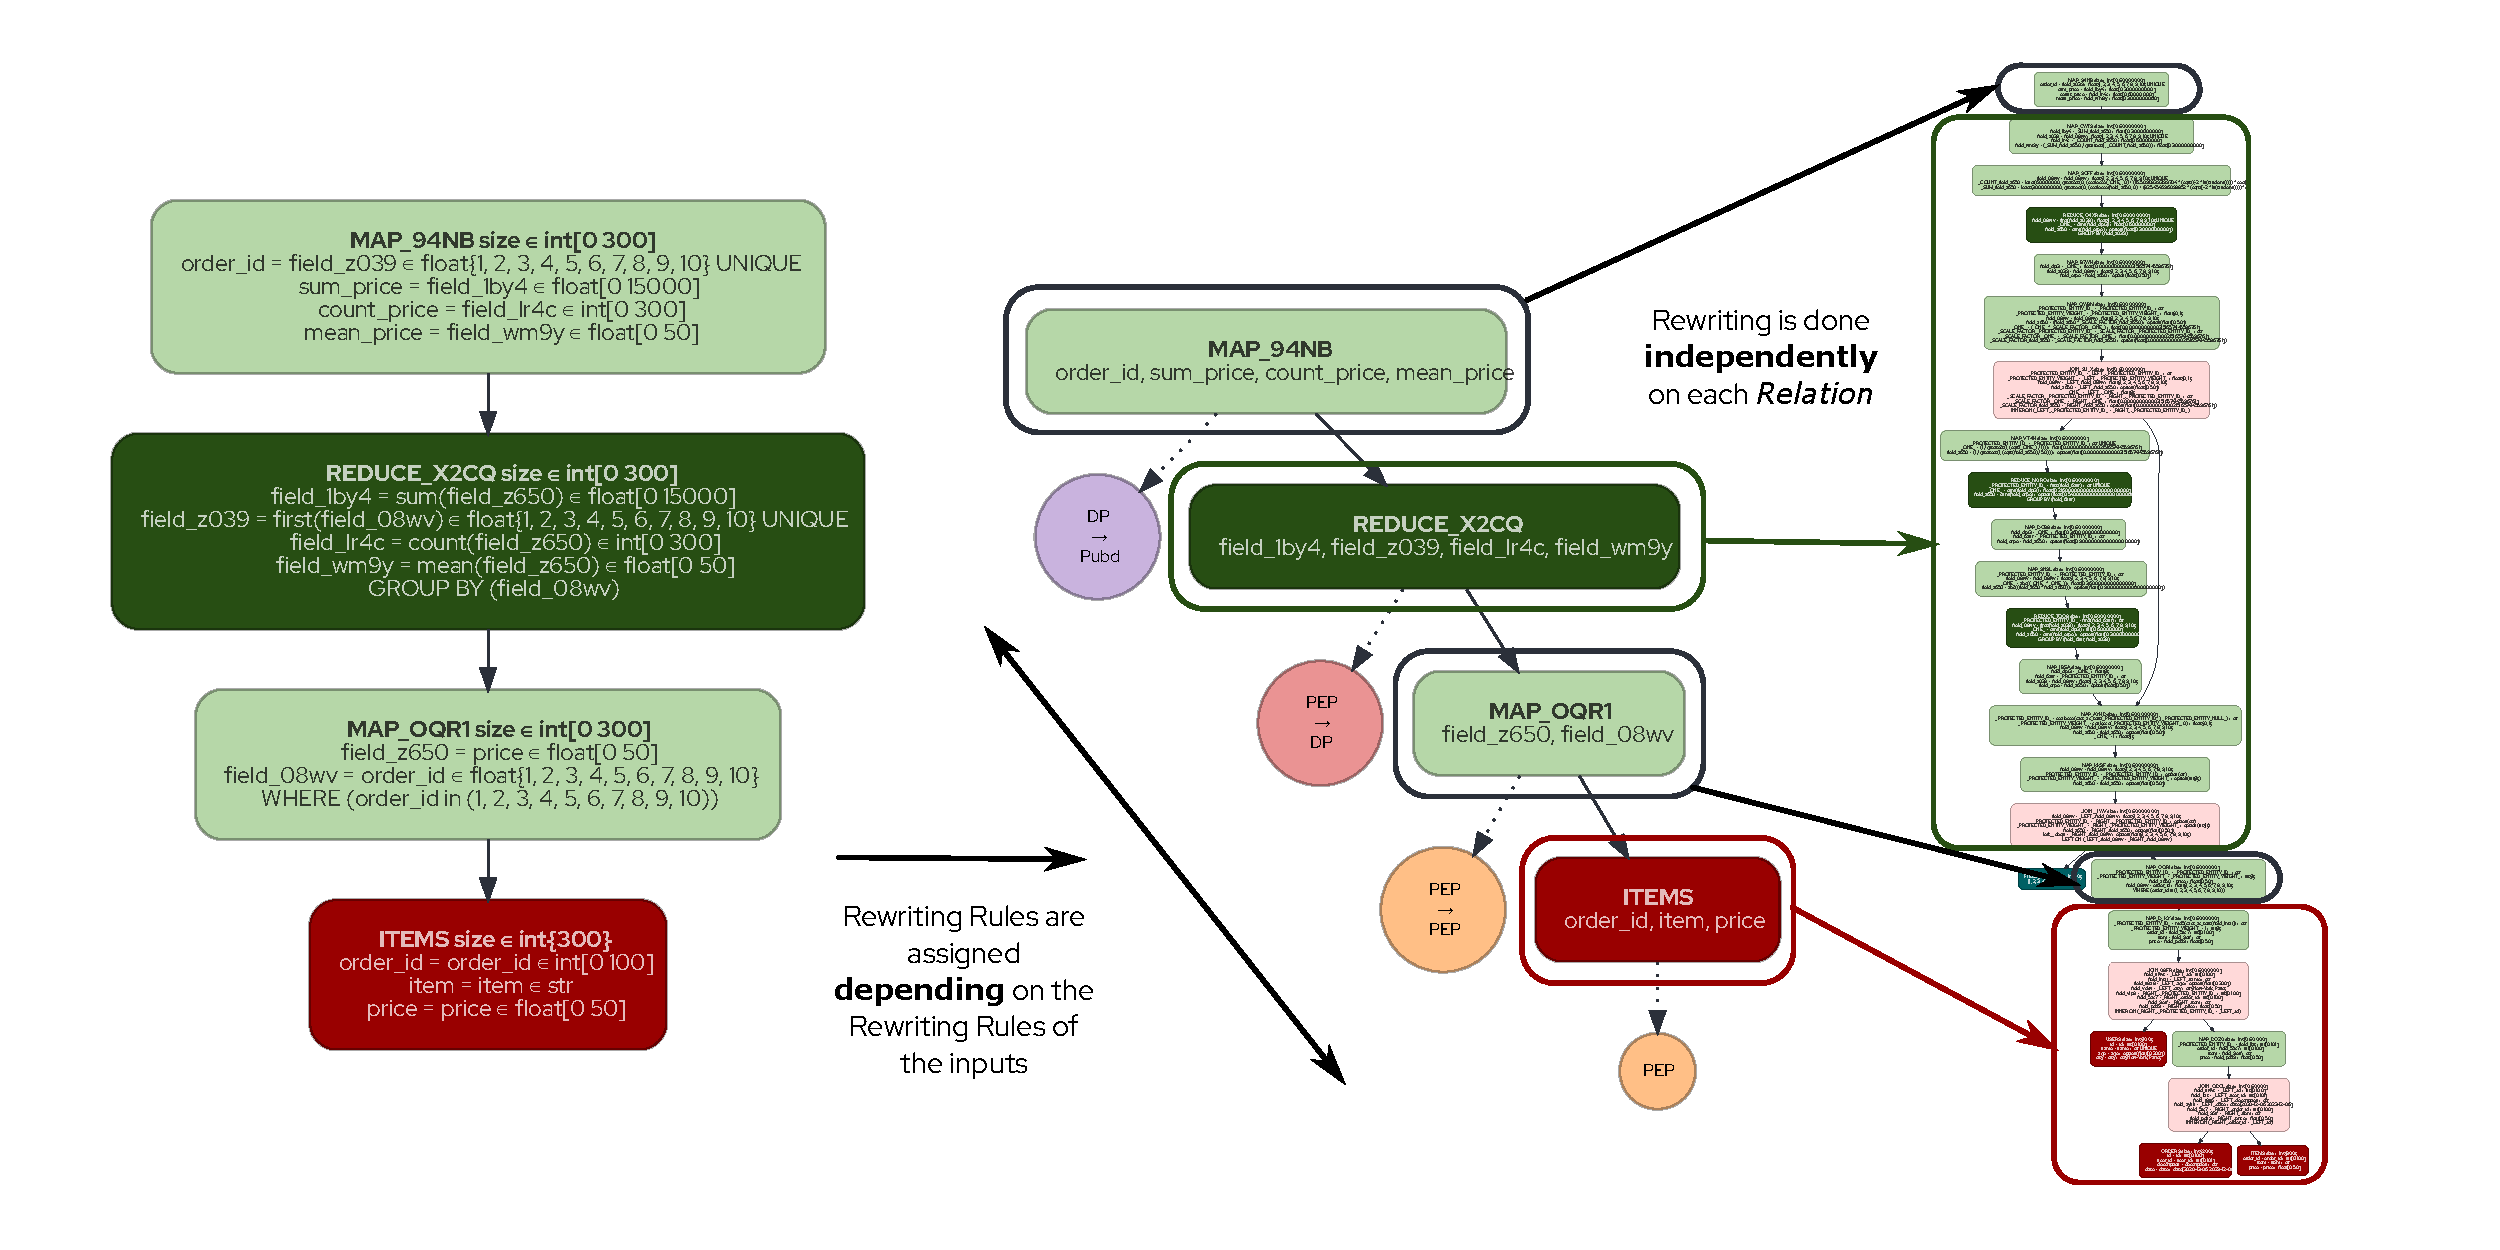
\includegraphics[width=0.9\textwidth]{figures/rewriting} % Reduce the figure size so that it is slightly narrower than the column.
    \caption{The rewriting process happens in two phases: a \emph{rewriting rule allocation} phase, where each node in the \emph{computation graph} gets allocated a \emph{rewriting rule} (RR) compatible with its input and with the desired output property; and a \emph{rule application} phase, where each \emph{Relation} is rewritten according to its allocated RR.}
    \label{fig:rewriting}
\end{figure*}

\subsubsection{Privacy Properties}
\label{sec:global_privacy_properties}
Let's sum up the global privacy properties:
\begin{itemize}
    \item \textbf{Protected Entity (PE)}: The definition of Differential Privacy (DP) is based on a notion of distance between datasets (see OpenDP work). Literature often formalizes datasets as multisets and uses the size of their symmetric difference as the distance between them (or equivalently, the $\ell_1$ norm of the difference of their histograms). In our clients' datasets, an individual's data is often described by several rows of data. To adapt the distance to this requirement, Sarus labels each data row with an identifier: the Protected Entity ID (PEID) and defines the distance between datasets as the size of the symmetric difference of the set of PEIDs from each dataset.
    \item \textbf{Protected Entity Preserving (PEP)}: A dataset is PEP if each data row is associated with a single PE. A dataset transformation is said to be PEP if each row labeled with a PEID results from calculations that do not depend on rows labeled with another PEID.
    \item \textbf{Differential Privacy (DP)}: A result will be qualified as DP if it comes from a DP mechanism applied to a PEP relation. A DP relation can be published if the associated privacy loss has been accurately accounted for.
    \item \textbf{Synthetic (SD)}: A relation derived only from transformation from the synthetic table.
    \item \textbf{Public (Pub)}: A relation derived from public tables is labeled as such and does not require DP protections.
    \item \textbf{Published (Pubd)}: A relation is considered 'published' if the overall mechanism from the private table to the relation complies with the differential privacy framework, ensuring that the privacy of the private data is maintained provided the dataset is not inherently public. This is achieved when all parent relations of a given relation are either published, public, synthetic themselves, or use a differential privacy mechanism.
\end{itemize}

\subsection{Rewriting Rule Allocation}

Rewriting rules are the main component to understand how to rewrite the computation graph. A rewriting rule is a local property explaining how to rewrite a relation to achieve global properties, being either DP, PEP, or synthetic, depending on some list of requirements on the privacy characteristics of the parents of the relation. In essence, a rewriting rule is a recursive step in the rewriting process. It explains how we could rewrite a relation given how we can rewrite the parents. The base case in the recursion is always: a table could either be private, public, or synthetic.

Relations can appear in various forms, including Join, Map, Reduce, Relation, Set, Table, and Values. Each type has its unique set of possible rewriting rules, outlining potential transformations and the associated global properties. An exhaustive list of the rewriting rules for each type of relation is provided in the annex.

\subsubsection{Key Rewriting Rules}

Let’s detail two crucial rewriting rules:

\paragraph{Relation with PEP \textrightarrow{} PEP and PEP \textrightarrow{} DP Rewriting Rules}
The first rule, PEP \textrightarrow{} PEP, concerns transferring the protected entity preserving property from one transformation stage to the next without mixing protected entities. The second rule, PEP \textrightarrow{} DP, means that if the parent of the relation can be rewritten as PEP, then we can rewrite the relation to be DP by applying a DP mechanism to publish the result. Both types of rewriting rules necessitate having parents that are capable of preserving protected entities. Some transformations, such as REDUCE, can aggregate data from multiple rows and thus can mix protected entities in the process. Such relations could be rewritten mostly only into published or synthetic, but it is possible that some REDUCE operations only aggregate rows related to the same protected entity and therefore could be rewritten into a PEP Relation.

\paragraph{Feasible Rewriting Rules}
A rewriting rule of a relation is said to be feasible if there exists a rewriting of the relation satisfying the rule. This is a global property of the relation, meaning that it depends on all the parents of the relation and not only on the transforms of the relation. Thus, the rewriting rule PEP \textrightarrow{} DP could be feasible for a relation if there exists a rewriting where the parent of the relation is in practice PEP. Then, we can change the transform and apply a DP mechanism to publish the relation. All rewriting rules about synthetic data are feasible because it is always possible in Sarus to build a synthetic variant of the relation using the synthetic table. The main goal of the DP rewriting is then to list for the relation that we want to obtain all the feasible rewriting rules and to select one where the outcome is DP. If not, it would mean that there does not exist a way to obtain this value using DP mechanisms, and we would need to use synthetic data.

\paragraph{Complexity of the Rewriting}
In the computation graph, while each node's multiple rewriting rules might suggest a combinatorial explosion in the number of possible paths, this is mitigated in practice. The pruning of infeasible rules, dictated by the requirement for most relations to have a PEP input for a DP or PEP outcome, significantly reduces the complexity. Hence, despite the theoretical breadth of possibilities, the actual number of feasible paths remains manageable, avoiding substantial computational problems.


\subsection{Implementation of the Rewriting Algorithm}

The goal is to have a deterministic algorithm that rewrites SQL queries into a privacy-preserving form. During the \qrlew{} rewriting process, the algorithm systematically goes through the computation graph, applying the following steps:

\begin{enumerate}
    \item Transform the SQL query into a computation graph composed of relations.
    \item Tagging rewriting rules: Initially tag all relations with their rewriting rules depending on the type of relation and the parameters of the relation from the list in the annex (see Figure~\ref{fig:rule_setting} for an illustration of Rule Setting).
    \item Filtering Out Infeasible Rules: Identify and remove recursively any rewriting rules that are not feasible, ensuring that only viable transformations are considered (refer to Figure~\ref{fig:rule_elimination} for a depiction of Rule Elimination).
    \item Applying Rewriting Rules: Starting from the last final node, for each node with multiple feasible rewriting rules, we select the best one based on a scoring system. The simple score system encodes the preferences among different privacy properties: we prefer to have a DP result than a synthetic one, that is why we give a better score for a feasible rule resulting in a DP result than a synthetic one (Figures~\ref{fig:sd_allocation} and \ref{fig:dp_allocation} illustrate examples of SD and DP Allocation, respectively).
    \item Building the Final Query: Once all relations have been transformed, convert the computation graph back into an SQL query that adheres to differential privacy standards. The budget is split among the different DP mechanisms involved in the computation graph.
\end{enumerate}




\section{Privacy Analysis}
\label{sec:privacy_algos}

At this stage, we examine a \texttt{Relation} that takes one or two protected \texttt{Relation} inputs, where the entity to be protected is specified.
To secure the outcome of the SQL query, it is imperative to protect not only the results obtained from aggregation functions but also the grouping keys.
We will briefly describe these two steps in the following section.

\subsubsection{Protecting aggregation results}

The protection of aggregation functions is carried out in three sequential steps. Given that all currently supported aggregations (\texttt{COUNT}, \texttt{SUM}, \texttt{AVG}, \texttt{VARIANCE} \texttt{STDDEV}) can be expressed as compositions of sums, our focus will be on the \texttt{SUM} aggregation. Let's consider the scenario where we aim to compute the sum of a column.

\begin{enumerate}
	\item \textbf{Limit the contribution per user within groups}:
	We represent the contribution of each user by a vector whose each component is the sum of the contributions within one group
    then we calculate its $\ell_2$ norm.
    Subsequently, we constrain the contributions of a specific user by scaling $\textbf{x}$ with a factor chosen to maintain the original observations if the $\ell_2$ norm of the user's observations does not exceed the clipping factor $c$.
    Conversely, if the $\ell_2$ norm surpasses $c$, the $\ell_2$  norm of the rescaled observations is restricted to $c$.
    More technical details can be found in the appendix \ref{sec:limit_contrib_per_user}.

	\item \textbf{Add random noise}:
	The sum of the original data is substituted with the sum of the scaled data with the addition of Gaussian noise. The level of noise is parameterized by the clipping and privacy parameters.

	\item \textbf{Restrict differentially private aggregation}:
	The final operation involves confining the differentially private aggregation within the bounds automatically computed for the $\text{\texttt{SUM}}(\textbf{x})$.
\end{enumerate}

\subsubsection{Protecting grouping keys}
As explained by \citeauthor{wilson2019differentially}, making grouping keys public could result in privacy breaches.
The treatment of grouping keys varies depending on whether the analyst knows them.

\begin{itemize}
	\item \textbf{Public Grouping Keys.}We categorize grouping keys as public when the analyst specifies them in the \texttt{WHERE} clause.
	In this scenario, all user-specified keys must be disclosed, even if they do not exist in the database.
	If a key is absent in the database, differentially private results will include these missing keys, and the corresponding aggregations will be random noise.
	\item \textbf{Revealing Private Keys through $\tau$-Thresholding}
	As introduced by \citeauthor{wilson2019differentially}, tau-thresholding involves releasing keys whose differentially private noise surpasses a threshold determined by privacy parameters.
\end{itemize}

When the SQL query involves both public and private grouping keys, we perform cross joins on the grouping keys obtained through the two algorithms.

\section{Comparison to other systems}

The Google Differential Privacy extension for PostgreSQL introduces differential privacy estimators for common aggregations like COUNT, SUM, AVG, STDDEV, and NTILE.
Despite its straightforward installation, using it can be challenging for non-experts.
While users can leverage the provided DP aggregations,
the privacy guarantees hold only if the user-supplied column and optional bounds meet the correct criteria (input column lies between the bounds and contains one line per user).
Constructing complex queries with Google DP can indeed be intricate, and users face uncertainties about privacy assurance,
especially when incorporating the protection of the grouping keys into the query.

OpenDP is a Rust library with Python bidings designed for building SQL-like analyses with differential privacy guarantees.
The framework provide many building blocks for building complex analysis with strong privacy guarantees.
Each part of the code is well documented with mathematical proofs but
its utilization can be challenging for non experts.
Besides this framework cannot be currently backed by an SQL database.

Similarly, Tumult Analytics doesn't directly process SQL queries but utilizes transformations that closely resemble SQL syntax.
These various implemented transformations provide users with the capability to construct more complex analyses,
leveraging the efficiency of Spark for computation.
However, it's essential to emphasize that the data owner has to run the analysis.

Smartnoise SQL is a Python framework for doing SQL analysis with differential privacy guarantees.
The framework is user-friendly for non-experts, but it does not support all SQL grammar such as complex queries with joins or subqueries.
Additionally, the execution of SQL analysis requires a Python post-processing step, potentially leading to increased execution times.

Chorus is the closest framework to \qrlew, and in the work by \citeauthor{johnson2020chorus},
there is a strong emphasis on conducting all analyses directly within the database.
However, it's worth noting that the code for Chorus is no longer being actively maintained.

\begin{table*}[h]
\centering
\begin{tabular}{|c|c|c|c|c|}
\hline
\textbf{System} & \textbf{SQL} & \textbf{Private joins}  & \textbf{Complex protected entity} & \textbf{DP guarantees on the result}\\
\hline
Google DP & \textcolor{green}{$\checkmark$} & \textcolor{red}{$\times$} &  \textcolor{red}{$\times$} & \textcolor{red}{$\times$} \\
\hline
Smartnoise SQL &  \textcolor{green}{\checkmark} & \textcolor{red}{$\times$} & \textcolor{red}{$\times$} & \textcolor{green}{$\checkmark$} \\
\hline
OpenDP & \textcolor{red}{$\times$} & \textcolor{red}{$\times$} & \textcolor{red}{$\times$} & \textcolor{green}{$\checkmark$} \\
\hline
Tumult Analytics &  \textcolor{red}{$\times$}&  \textcolor{green}{\checkmark} &  \textcolor{green}{\checkmark} & \textcolor{green}{$\checkmark$} \\
\hline
Chorus & \textcolor{green}{\checkmark} & \textcolor{green}{\checkmark} &  \textcolor{red}{$\times$} & \textcolor{green}{$\checkmark$}\\
\hline
Qrlew &  \textcolor{green}{\checkmark}&  \textcolor{green}{\checkmark}&  \textcolor{green}{\checkmark}&  \textcolor{green}{\checkmark} \\
\hline
\end{tabular}
\caption{
    Systems Comparison.
    This table contrasts various open-source models designed for SQL-like analysis. The columns indicate different features:
    \textbf{SQL} denotes whether the input is an SQL query,
    \textbf{Private Joins} signifies systems that automatically rewrite joins into differential privacy (DP),
    \textbf{Complex Protected Entity} indicates the system's ability to handle non-trivial protected entities, such as columns from another table,
    and \textbf{DP Guarantees on the Result} specifies systems providing differential privacy guarantees on the analysis results.t
}
\label{table:systems}
\end{table*}

\section{Known limitations}

\qrlew{} relies on the random number generator of the SQL engine used. It is usually not a cryptographic noise.

\qrlew{} uses the floating-point numbers of the host SQL engine, therefore our system is liable to the vulnerabilities described in \citeauthor{casacuberta2022widespread}.


\section*{Useful links}
\subsection{PPAI}
Last year papers:
\url{https://aaai-ppai23.github.io/#sp2}
This year program:
\url{https://ppai-workshop.github.io/}

\subsection{Comparable open-source projects}

\begin{itemize}
    \item Paszke et al. 2017 - Automatic differentiation in PyTorch \url{https://openreview.net/pdf?id=BJJsrmfCZ}
    \item Frostig et al. 2018 - Compiling machine learning programs via high-level tracing \url{https://mlsys.org/Conferences/2019/doc/2018/146.pdf}
\end{itemize}

\subsection{Comparable DP SQL papers}

\begin{itemize}
    \item Lessons Learned: Surveying the Practicality of Differential Privacy in the Industry \cite{garrido2022lessons}
    \item Tumult Analytics: a robust, easy-to-use, scalable, and expressive framework for differential privacy \cite{berghel2022tumult}
    \item Differentially Private SQL with Bounded User Contribution \cite{wilson2019differentially}
    \item CHORUS: a Programming Framework for Building Scalable Differential Privacy Mechanisms \cite{johnson2020chorus}
    \item Towards Practical Differential Privacy for SQL Queries \cite{johnson2018towards}
\end{itemize}

\bigskip
\noindent Thank you for reading these instructions carefully. We look forward to receiving your electronic files!

% \bibliography{aaai24}
\bibliography{qrlew}
\appendix

\section*{Appendix}

\begin{figure*}[t]
    \centering
    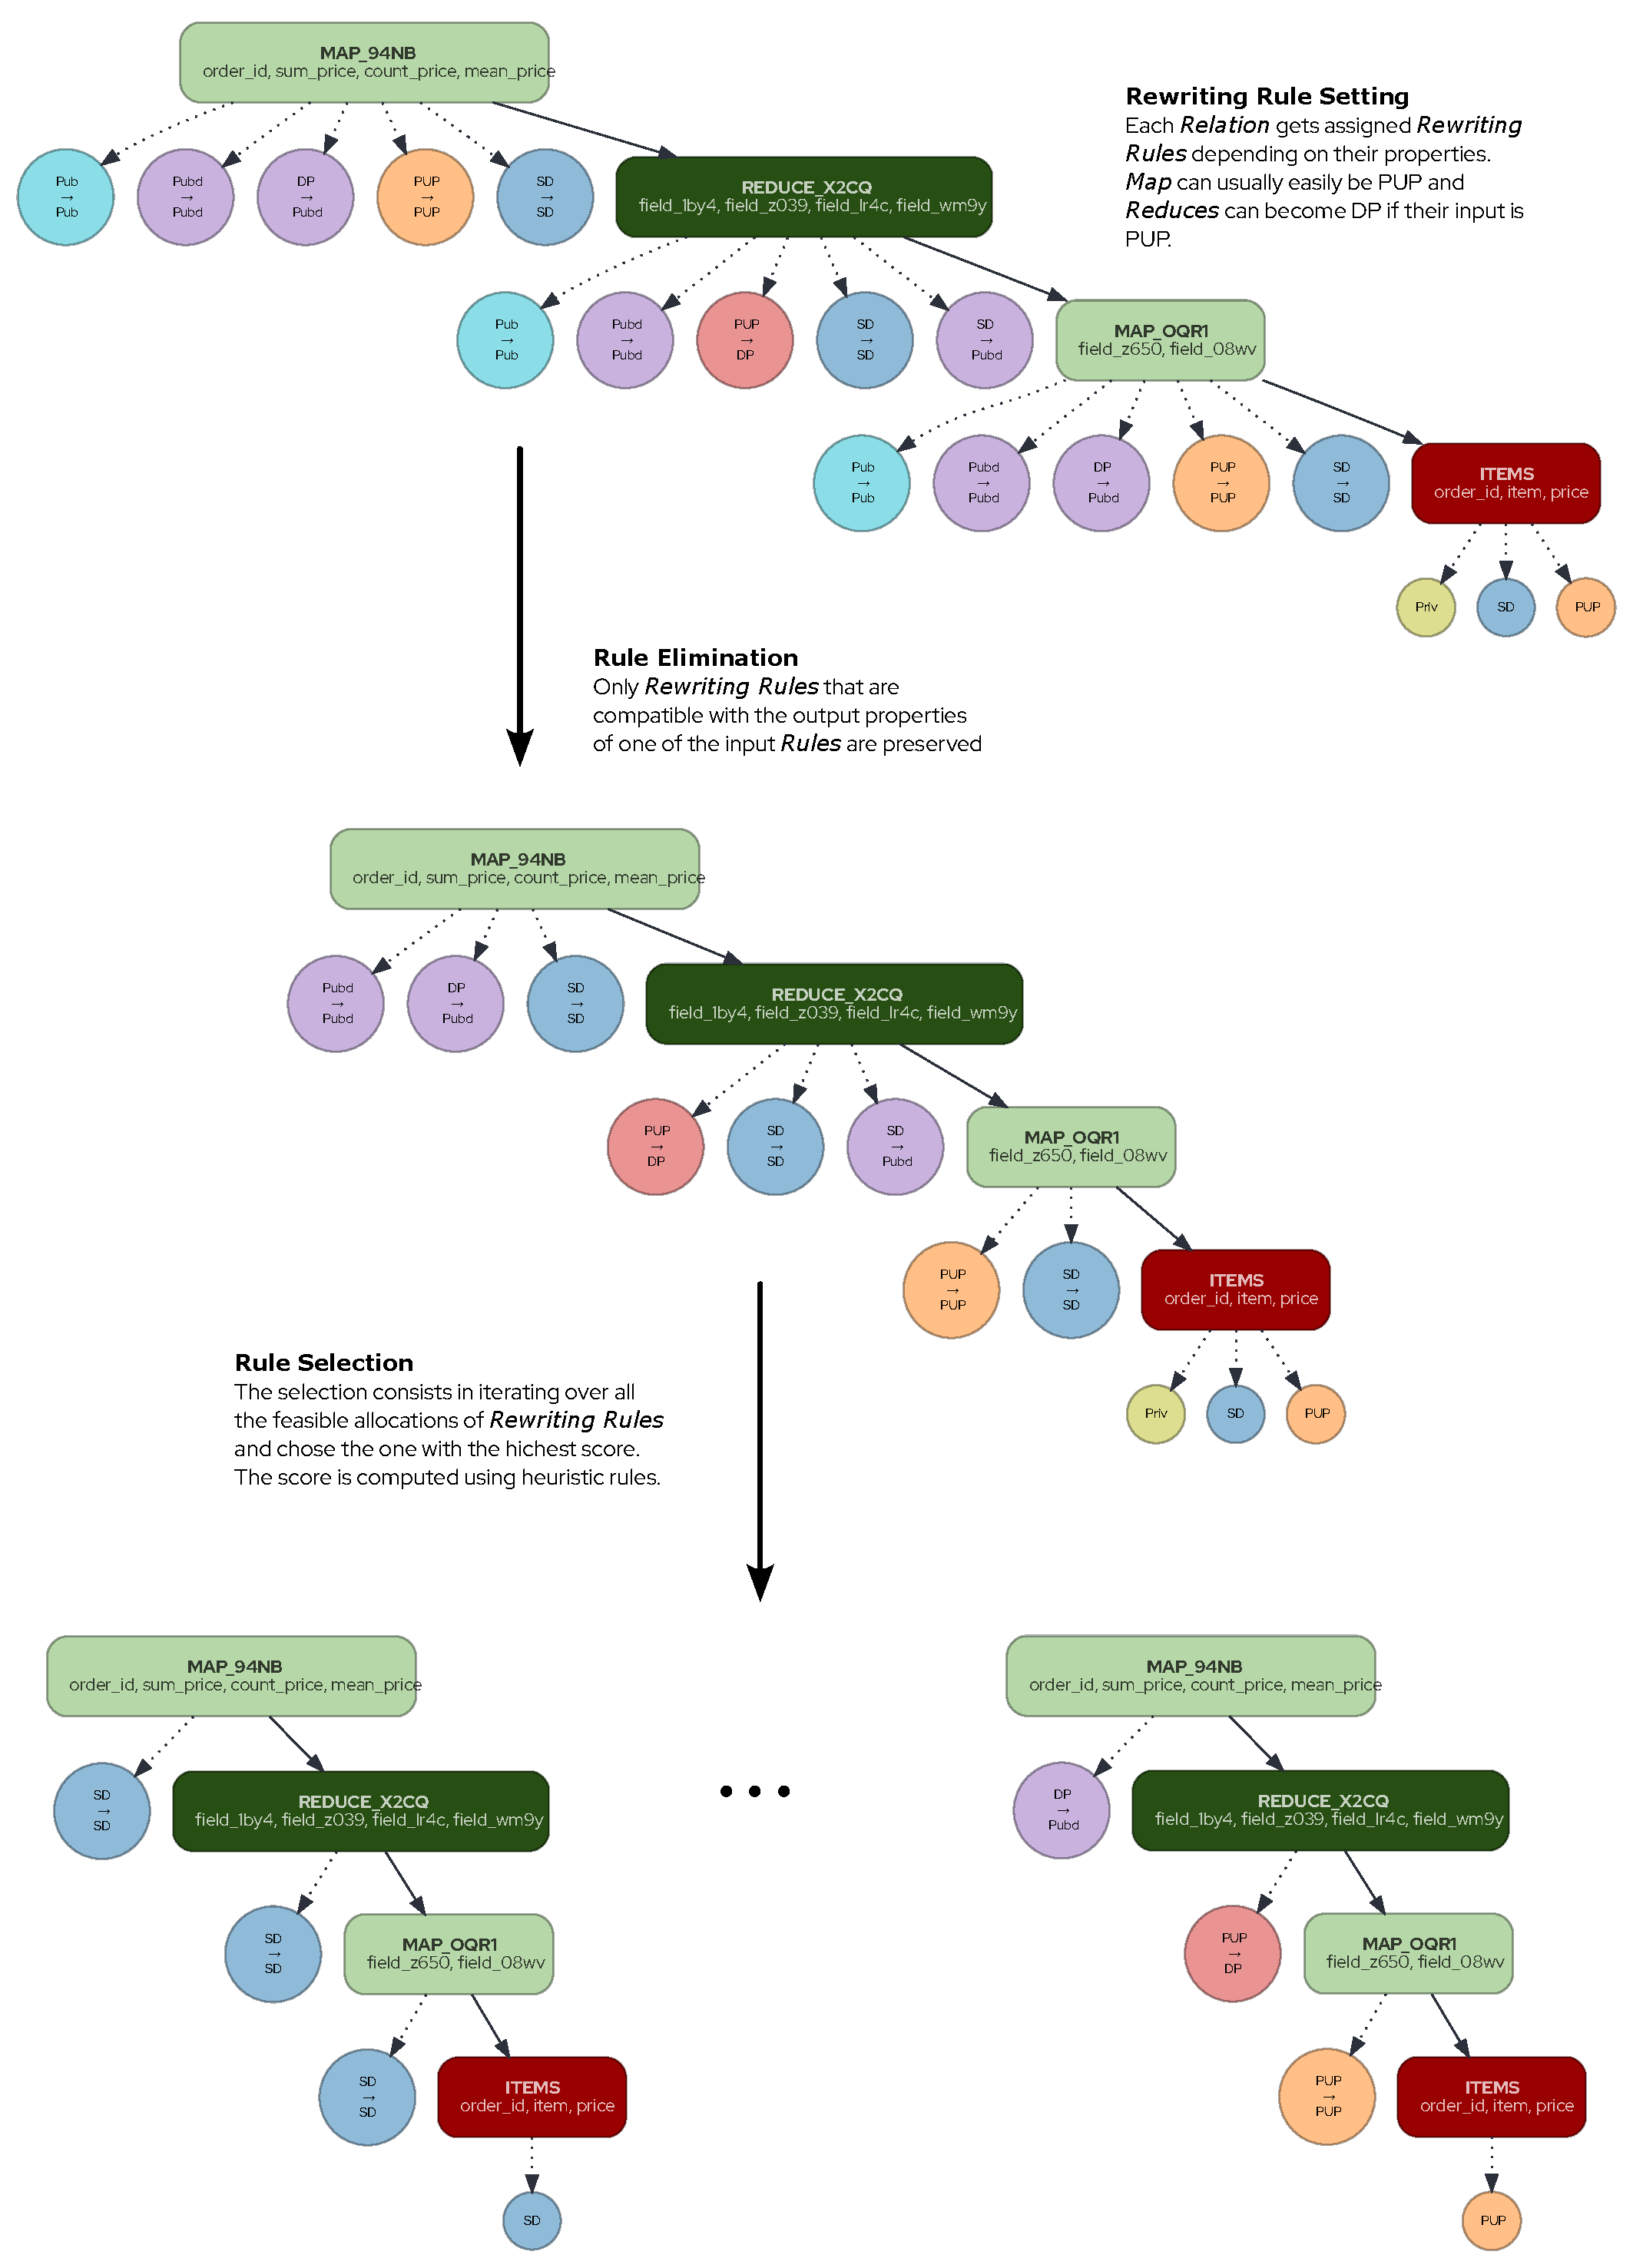
\includegraphics[width=0.9\textwidth]{figures/set_eliminate_select} % Reduce the figure size so that it is slightly narrower than the column.
    \caption{The rewriting happens in thress steps}
    \label{fig:set_eliminate_select}
\end{figure*}


\section*{Appendix: Limit the contribution per user within the aggregations}
\label{sec:limit_contrib_per_user}

The observations can be represented as a matrix whose first dimension is the user
and second dimension is the group:

\[ \vphantom{% phantom stuff for correct box dimensions
    \begin{matrix}
    \overbrace{XYZ}^{\mbox{$R$}}\\ \\ \\ \\ \\ \\
    \end{matrix}}%
\begin{pmatrix}
    \coolover{\text{Group 1}}{~~~x_{11}} & \coolover{\text{Group 2}}{~~~x_{12}} & \hdots & \coolover{\text{Group n}}{~~~x_{1n}} \\
    ~~~x_{21} & ~~~x_{22} & \hdots & ~~~x_{2n}  \\
    \vdots & \vdots &  & \vdots  \\
    ~~~x_{m1} & ~~~x_{m2} & \hdots & ~~~x_{mn}
\end{pmatrix}%
\begin{matrix}% matrix for right braces
    \coolrightbrace{x}{\text{User 1}}\\
    \coolrightbrace{x}{\text{User 2}}\\
    \vphantom{\vdots} \\
    \coolrightbrace{x}{\text{User }m}\\
\end{matrix}
\]

The coordinate $x_{ij}$ is the sum of all the observations of user $i$ within the group $j$.


For each user $i$, we compute the scale factor that constrains his contribution to a maximum value of $c$:

\begin{equation}
	s_i = \frac{1}{\max ( 1, \frac{1}{c} \ell_2(x_{i,.}) )} \text{  with  } \ell_2(x_{i,.}) = \sqrt{\sum_j x^2_{ij}}.
\end{equation}

The original data is then rescaled by multiplying each observation by the corresponding user's scale factor.
This process ensures that the $\ell_2$ contribution of each user is restricted to $c$ within the rescaled data.

In our algorithm, the clipping value $c$ is given by:
\begin{equation}
    c = \max ( |\min \textbf{x}|, |\max \textbf{x}|),
\end{equation}
where $\min \textbf{x}$ and $\max \textbf{x}$ are the automatically computed bounds of $\textbf{x}$.

\bigskip
\subsection*{Description of the Rewriting Rules for Each Type of Relation}
\label{sec:rewriting_rules}

\subsubsection*{Map Function: Transforming a Single Relation}
\begin{itemize}
    \item Pub \textrightarrow{} Pub: A relation could stay public if it starts off public.
    \item Pubd \textrightarrow{} Pubd: A relation could stay published if it starts off published.
    \item PEP \textrightarrow{} DP (with specific budget): A relation could become differentially private, adopting a specific budget, if it starts off preserving protected entities.
    \item SD \textrightarrow{} SD: A relation could remain as synthetic data if it starts off as synthetic data.
    \item SD \textrightarrow{} Pubd (with specific synthetic data parameters): A relation could transform into published if it starts off as synthetic data, depending on specific synthetic data parameters.
\end{itemize}

\subsubsection*{Reduce Function: Transforming a Single Relation}
\begin{itemize}
    \item Pub \textrightarrow{} Pub: A relation could stay public if its parent is public.
    \item Pubd \textrightarrow{} Pubd: A relation could stay published if its parent is published.
    \item PEP \textrightarrow{} DP (with specific budget): A relation could become differentially private, adopting a specific budget, if it is preserving protected entities.
    \item SD \textrightarrow{} SD: A relation could remain as synthetic data if its parent is synthetic data.
    \item SD \textrightarrow{} Pubd (with specific synthetic data parameters): A relation could transform into published if it is synthetic data, depending on specific synthetic data parameters.
\end{itemize}

\subsubsection*{Join Function: Combining Two Relations}
\begin{itemize}
    \item Pub + Pub \textrightarrow{} Pub: Combining two public relations could result in a public relation.
    \item Pubd + Pubd \textrightarrow{} Pubd: Combining two published relations could result in a published relation.
    \item Pubd + PEP \textrightarrow{} PEP (with specific parameters): Combining a published relation and a relation that preserves protected entities could result in a relation that preserves protected entities, adopting specific parameters.
    \item PEP + PEP \textrightarrow{} PEP (with specific parameters): Combining two relations that preserve protected entities could result in a relation that preserves protected entities, adopting specific parameters.
    \item DP + PEP \textrightarrow{} PEP (with specific parameters): Combining a differentially private relation and a relation that preserves protected entities could result in a relation that preserves protected entities, adopting specific parameters.
    \item SD + SD \textrightarrow{} SD: Combining two synthetic data relations could result in a synthetic data relation.
\end{itemize}

\subsubsection*{Set Function: Merging Two Relations}
\begin{itemize}
    \item Pub + Pub \textrightarrow{} Pub: Combining two public relations could result in a public relation.
    \item Pubd + Pubd \textrightarrow{} Pubd: Combining two published relations could result in a published relation.
    \item PEP + PEP \textrightarrow{} PEP (with specific parameters): Combining two relations that preserve protected entities could result in a relation that preserves protected entities, adopting specific parameters.
    \item SD + SD \textrightarrow{} SD (with specific parameters): Combining two synthetic data relations could result in a synthetic data relation, adopting specific parameters.
\end{itemize}

\subsubsection*{Values Function: Creating a New Relation}
\begin{itemize}
    \item \textrightarrow{} SD (with specific parameters): A new relation could be created as synthetic data, depending on specific parameters.
    \item \textrightarrow{} Pub: A new relation could be created as public.
\end{itemize}

\bigskip
\subsection*{Visual Depiction of Algorithmic Steps}
\label{sec:graphviz}

The computation graph figures illustrate the step-by-step transformation of relations within \qrlew{}. The rectangles (relations) represent tables or intermediate results, and the circles represent the rewriting rules (feasible or not) of these relations. Here is how to understand the components and read the figures:

\begin{itemize}
    \item \textbf{Rectangles} symbolize the relations in the computation graph, which could be a base table or derived through operations such as Join, Map, Reduce, etc.
    \item \textbf{Circles} denote the rewriting rules that can be applied to these relations. The color and label of each circle indicate the type of rewriting rule:
    \item The \textbf{arrows} connecting the circles to the rectangles show which rewriting rules can be applied to which relations.
    \item A sequence of transformations is shown as a path through the graph, beginning with the source relations at the bottom and culminating in the final transformed query at the top.
\end{itemize}


\end{document}
